\documentclass[11pt,preprint, authoryear]{elsarticle}

\usepackage{lmodern}
%%%% My spacing
\usepackage{setspace}
\setstretch{1.2}
\DeclareMathSizes{12}{14}{10}{10}

% Wrap around which gives all figures included the [H] command, or places it "here". This can be tedious to code in Rmarkdown.
\usepackage{float}
\let\origfigure\figure
\let\endorigfigure\endfigure
\renewenvironment{figure}[1][2] {
    \expandafter\origfigure\expandafter[H]
} {
    \endorigfigure
}

\let\origtable\table
\let\endorigtable\endtable
\renewenvironment{table}[1][2] {
    \expandafter\origtable\expandafter[H]
} {
    \endorigtable
}


\usepackage{ifxetex,ifluatex}
\usepackage{fixltx2e} % provides \textsubscript
\ifnum 0\ifxetex 1\fi\ifluatex 1\fi=0 % if pdftex
  \usepackage[T1]{fontenc}
  \usepackage[utf8]{inputenc}
\else % if luatex or xelatex
  \ifxetex
    \usepackage{mathspec}
    \usepackage{xltxtra,xunicode}
  \else
    \usepackage{fontspec}
  \fi
  \defaultfontfeatures{Mapping=tex-text,Scale=MatchLowercase}
  \newcommand{\euro}{€}
\fi

\usepackage{amssymb, amsmath, amsthm, amsfonts}

\def\bibsection{\section*{References}} %%% Make "References" appear before bibliography


\usepackage[round]{natbib}

\usepackage{longtable}
\usepackage[margin=2.3cm,bottom=2cm,top=2.5cm, includefoot]{geometry}
\usepackage{fancyhdr}
\usepackage[bottom, hang, flushmargin]{footmisc}
\usepackage{graphicx}
\numberwithin{equation}{section}
\numberwithin{figure}{section}
\numberwithin{table}{section}
\setlength{\parindent}{0cm}
\setlength{\parskip}{1.3ex plus 0.5ex minus 0.3ex}
\usepackage{textcomp}
\renewcommand{\headrulewidth}{0.2pt}
\renewcommand{\footrulewidth}{0.3pt}

\usepackage{array}
\newcolumntype{x}[1]{>{\centering\arraybackslash\hspace{0pt}}p{#1}}

%%%%  Remove the "preprint submitted to" part. Don't worry about this either, it just looks better without it:
\makeatletter
\def\ps@pprintTitle{%
  \let\@oddhead\@empty
  \let\@evenhead\@empty
  \let\@oddfoot\@empty
  \let\@evenfoot\@oddfoot
}
\makeatother

 \def\tightlist{} % This allows for subbullets!

\usepackage{hyperref}
\hypersetup{breaklinks=true,
            bookmarks=true,
            colorlinks=true,
            citecolor=blue,
            urlcolor=blue,
            linkcolor=blue,
            pdfborder={0 0 0}}


% The following packages allow huxtable to work:
\usepackage{siunitx}
\usepackage{multirow}
\usepackage{hhline}
\usepackage{calc}
\usepackage{tabularx}
\usepackage{booktabs}
\usepackage{caption}


\newenvironment{columns}[1][]{}{}

\newenvironment{column}[1]{\begin{minipage}{#1}\ignorespaces}{%
\end{minipage}
\ifhmode\unskip\fi
\aftergroup\useignorespacesandallpars}

\def\useignorespacesandallpars#1\ignorespaces\fi{%
#1\fi\ignorespacesandallpars}

\makeatletter
\def\ignorespacesandallpars{%
  \@ifnextchar\par
    {\expandafter\ignorespacesandallpars\@gobble}%
    {}%
}
\makeatother

\newlength{\cslhangindent}
\setlength{\cslhangindent}{1.5em}
\newenvironment{CSLReferences}%
  {\setlength{\parindent}{0pt}%
  \everypar{\setlength{\hangindent}{\cslhangindent}}\ignorespaces}%
  {\par}


\urlstyle{same}  % don't use monospace font for urls
\setlength{\parindent}{0pt}
\setlength{\parskip}{6pt plus 2pt minus 1pt}
\setlength{\emergencystretch}{3em}  % prevent overfull lines
\setcounter{secnumdepth}{5}

%%% Use protect on footnotes to avoid problems with footnotes in titles
\let\rmarkdownfootnote\footnote%
\def\footnote{\protect\rmarkdownfootnote}
\IfFileExists{upquote.sty}{\usepackage{upquote}}{}

%%% Include extra packages specified by user

%%% Hard setting column skips for reports - this ensures greater consistency and control over the length settings in the document.
%% page layout
%% paragraphs
\setlength{\baselineskip}{12pt plus 0pt minus 0pt}
\setlength{\parskip}{12pt plus 0pt minus 0pt}
\setlength{\parindent}{0pt plus 0pt minus 0pt}
%% floats
\setlength{\floatsep}{12pt plus 0 pt minus 0pt}
\setlength{\textfloatsep}{20pt plus 0pt minus 0pt}
\setlength{\intextsep}{14pt plus 0pt minus 0pt}
\setlength{\dbltextfloatsep}{20pt plus 0pt minus 0pt}
\setlength{\dblfloatsep}{14pt plus 0pt minus 0pt}
%% maths
\setlength{\abovedisplayskip}{12pt plus 0pt minus 0pt}
\setlength{\belowdisplayskip}{12pt plus 0pt minus 0pt}
%% lists
\setlength{\topsep}{10pt plus 0pt minus 0pt}
\setlength{\partopsep}{3pt plus 0pt minus 0pt}
\setlength{\itemsep}{5pt plus 0pt minus 0pt}
\setlength{\labelsep}{8mm plus 0mm minus 0mm}
\setlength{\parsep}{\the\parskip}
\setlength{\listparindent}{\the\parindent}
%% verbatim
\setlength{\fboxsep}{5pt plus 0pt minus 0pt}



\begin{document}



\begin{frontmatter}  %

\title{What Caused The Early Millenium Slowdown? Evidenece Based on
Vector Autoregressions}

% Set to FALSE if wanting to remove title (for submission)




\author[Add1]{Jessica Van der Berg}
\ead{20190565@sun.ac.za}





\address[Add1]{20190565}


\begin{abstract}
\small{
Abstract to be written here. The abstract should not be too long and
should provide the reader with a good understanding what you are writing
about. Academic papers are not like novels where you keep the reader in
suspense. To be effective in getting others to read your paper, be as
open and concise about your findings here as possible. Ideally, upon
reading your abstract, the reader should feel he / she must read your
paper in entirety.
}
\end{abstract}

\vspace{1cm}

\begin{keyword}
\footnotesize{
Multivariate GARCH \sep Kalman Filter \sep Copula \\ \vspace{0.3cm}
\textit{JEL classification} L250 \sep L100
}
\end{keyword}
\vspace{0.5cm}
\end{frontmatter}



%________________________
% Header and Footers
%%%%%%%%%%%%%%%%%%%%%%%%%%%%%%%%%
\pagestyle{fancy}
\chead{}
\rhead{A replication of Gert Peersman (2005) paper}
\lfoot{}
\rfoot{\footnotesize Page \thepage}
\lhead{}
%\rfoot{\footnotesize Page \thepage } % "e.g. Page 2"
\cfoot{}

%\setlength\headheight{30pt}
%%%%%%%%%%%%%%%%%%%%%%%%%%%%%%%%%
%________________________

\headsep 35pt % So that header does not go over title




\hypertarget{test-wether-variables-are-stationary}{%
\section{\texorpdfstring{Test wether variables are stationary
\label{stationary}}{Test wether variables are stationary }}\label{test-wether-variables-are-stationary}}

Variables that are included in the dataset (same order): oil, output
growth, consumer inflation and short-term nominal interest rate for EU
and US.

Gideon suggested I only do the replication for the US, since this will
be a lot of work.

In order to test whether a variable is stationary, you can use a unit
root test such as the Dickey-Fuller (DF) test

Null hypothesis: There is a unit root Alternative hypothesis: Time
series is stationary

If p-values is less than 0.05, it means we can reject the null
hypothesis.

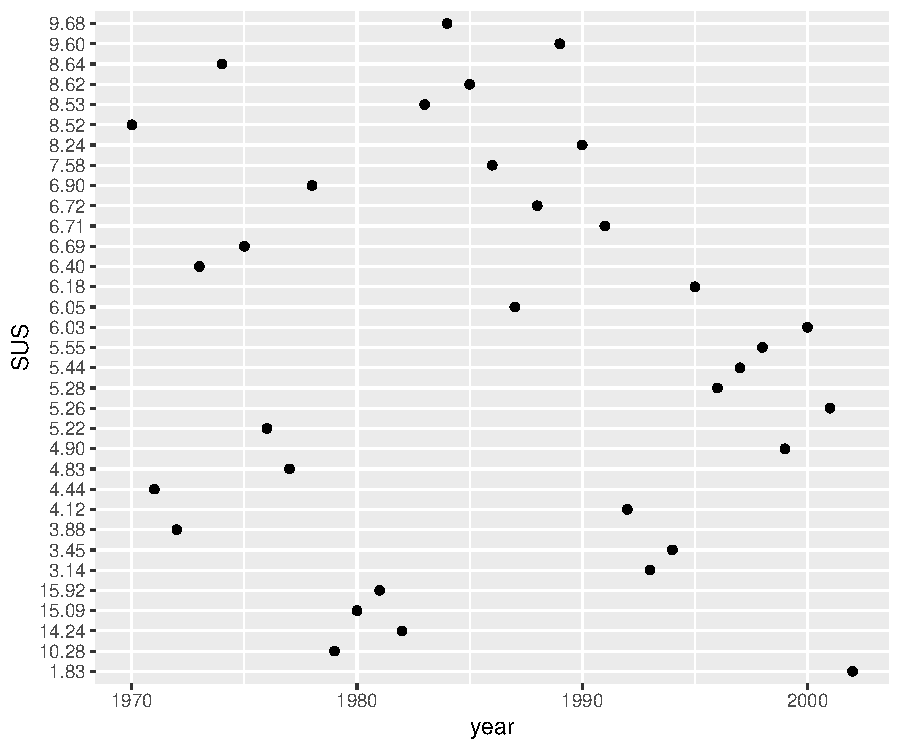
\includegraphics{replication_files/figure-latex/unnamed-chunk-1-1.pdf}

\begin{verbatim}
## 
##  Augmented Dickey-Fuller Test
## 
## data:  slowdown_dataset$OIL
## Dickey-Fuller = -2.0358, Lag order = 5, p-value = 0.5616
## alternative hypothesis: stationary
\end{verbatim}

\begin{verbatim}
## 
##  Augmented Dickey-Fuller Test
## 
## data:  slowdown_dataset$YUS
## Dickey-Fuller = -1.3894, Lag order = 5, p-value = 0.8304
## alternative hypothesis: stationary
\end{verbatim}

\begin{verbatim}
## 
##  Augmented Dickey-Fuller Test
## 
## data:  slowdown_dataset$SUS
## Dickey-Fuller = -3.4394, Lag order = 5, p-value = 0.05113
## alternative hypothesis: stationary
\end{verbatim}

\begin{verbatim}
## 
##  Augmented Dickey-Fuller Test
## 
## data:  slowdown_dataset$CPUS
## Dickey-Fuller = -1.5413, Lag order = 5, p-value = 0.7672
## alternative hypothesis: stationary
\end{verbatim}

\begin{verbatim}
## 
##  Phillips-Perron Unit Root Test
## 
## data:  slowdown_dataset$OIL
## Dickey-Fuller Z(alpha) = -8.7804, Truncation lag parameter = 4, p-value
## = 0.6091
## alternative hypothesis: stationary
\end{verbatim}

\begin{verbatim}
## 
##  Phillips-Perron Unit Root Test
## 
## data:  slowdown_dataset$YUS
## Dickey-Fuller Z(alpha) = -3.501, Truncation lag parameter = 4, p-value
## = 0.9108
## alternative hypothesis: stationary
\end{verbatim}

\begin{verbatim}
## 
##  Phillips-Perron Unit Root Test
## 
## data:  slowdown_dataset$SUS
## Dickey-Fuller Z(alpha) = -11.903, Truncation lag parameter = 4, p-value
## = 0.4288
## alternative hypothesis: stationary
\end{verbatim}

\begin{verbatim}
## 
##  Phillips-Perron Unit Root Test
## 
## data:  slowdown_dataset$CPUS
## Dickey-Fuller Z(alpha) = -1.0566, Truncation lag parameter = 4, p-value
## = 0.9855
## alternative hypothesis: stationary
\end{verbatim}

\hypertarget{optimal-lag-length}{%
\section{Optimal lag length}\label{optimal-lag-length}}

I now determine the optimal lag length for an unrestricted VAR with a
maximum lag length of 10.

According to the AIC and the FPE, the optimal lag length is 4. However,
the SC and HQ criterion indicates an optimal lag length of 1. The data
estimates a VAR including a constant and a trend as deterministic
regressor.

I will use a VAR with lag length eual to one as specified by the paper.

\begin{verbatim}
## $selection
## AIC(n)  HQ(n)  SC(n) FPE(n) 
##      4      1      1      4 
## 
## $criteria
##                   1            2            3           4           5
## AIC(n)     9.388028     9.276473     9.256966    9.110758     9.33497
## HQ(n)      9.614431     9.653811     9.785239    9.789965    10.16511
## SC(n)      9.945526    10.205637    10.557796   10.783253    11.37913
## FPE(n) 11948.510504 10700.252306 10522.129466 9135.114589 11518.86905
##                  6            7            8            9           10
## AIC(n)     9.47171     9.679419     9.682826     9.802003     9.872561
## HQ(n)     10.45279    10.811433    10.965774    11.235887    11.457380
## SC(n)     11.88754    12.466911    12.841983    13.332826    13.775050
## FPE(n) 13354.70319 16692.619524 17095.671652 19774.982422 21940.976772
\end{verbatim}

\hypertarget{var}{%
\section{VAR}\label{var}}

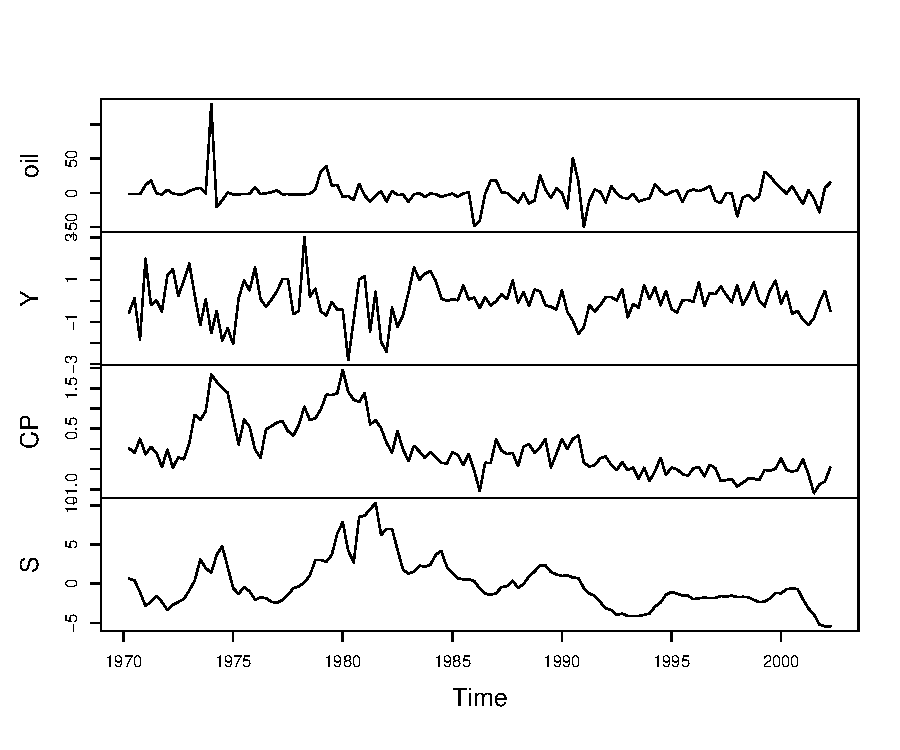
\includegraphics{replication_files/figure-latex/unnamed-chunk-3-1.pdf}
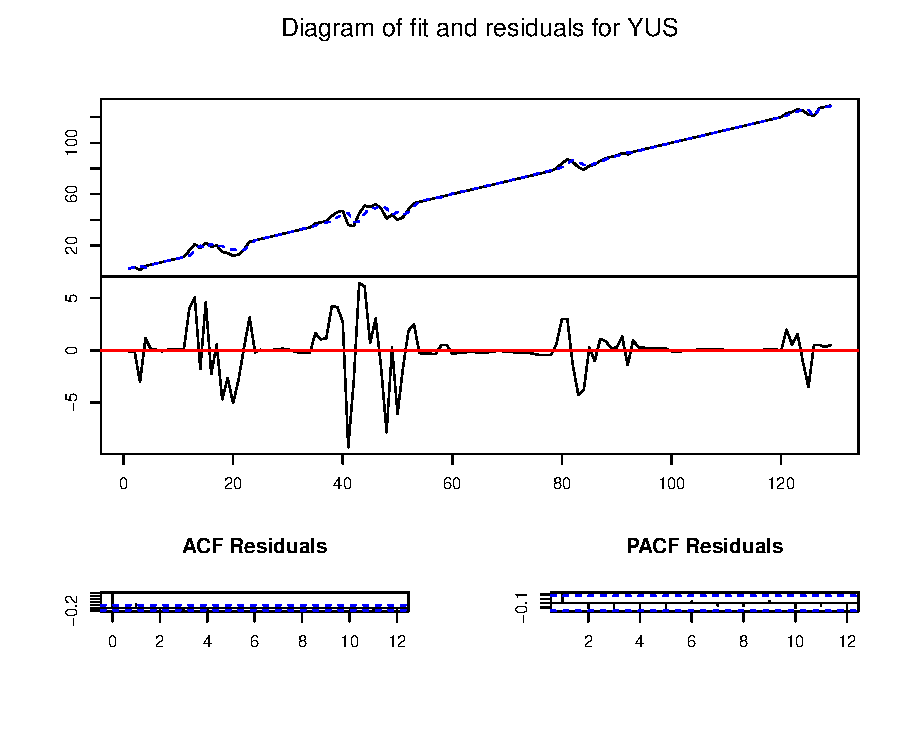
\includegraphics{replication_files/figure-latex/unnamed-chunk-3-2.pdf}
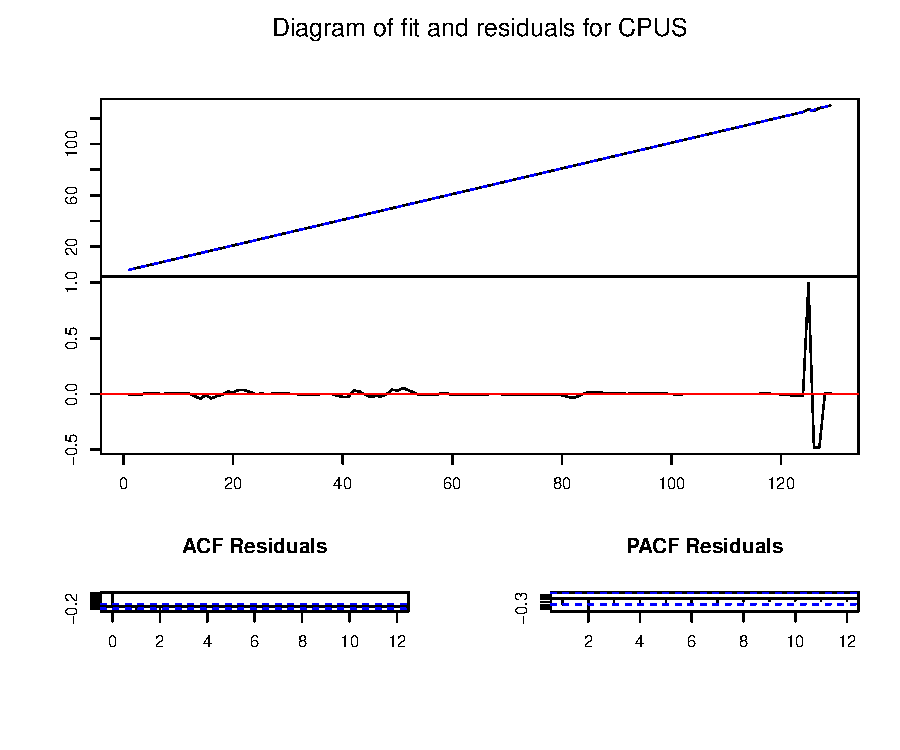
\includegraphics{replication_files/figure-latex/unnamed-chunk-3-3.pdf}
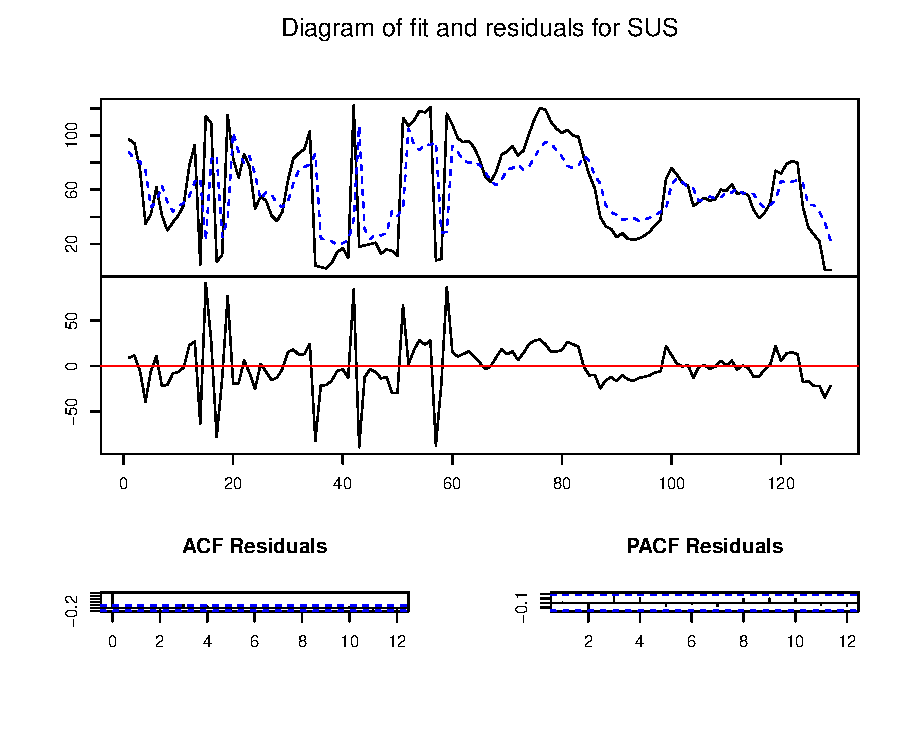
\includegraphics{replication_files/figure-latex/unnamed-chunk-3-4.pdf}

\hypertarget{diagnostic-tests-and-test-statistics}{%
\section{Diagnostic tests and Test
statistics}\label{diagnostic-tests-and-test-statistics}}

The results for diagnostic test for VAR(1), VAR(2) and VAR(3) are
provided in the table below.

Here you look and interpret all the test to determine whether VAR(1) is
too restrictive. ARGUE this as part of your robustness test for the
paper.

\begin{verbatim}
## 
##  Portmanteau Test (asymptotic)
## 
## data:  Residuals of VAR object VAR(ts_us, p = 1, type = "both")
## Chi-squared = 212.62, df = 240, p-value = 0.898
\end{verbatim}

\begin{verbatim}
## $JB
## 
##  JB-Test (multivariate)
## 
## data:  Residuals of VAR object VAR(ts_us, p = 1, type = "both")
## Chi-squared = 18850, df = 8, p-value < 2.2e-16
## 
## 
## $Skewness
## 
##  Skewness only (multivariate)
## 
## data:  Residuals of VAR object VAR(ts_us, p = 1, type = "both")
## Chi-squared = 472.22, df = 4, p-value < 2.2e-16
## 
## 
## $Kurtosis
## 
##  Kurtosis only (multivariate)
## 
## data:  Residuals of VAR object VAR(ts_us, p = 1, type = "both")
## Chi-squared = 18377, df = 4, p-value < 2.2e-16
\end{verbatim}

\begin{verbatim}
## 
##  ARCH (multivariate)
## 
## data:  Residuals of VAR object VAR(ts_us, p = 1, type = "both")
## Chi-squared = 786.65, df = 500, p-value = 3.886e-15
\end{verbatim}

\hypertarget{impulse-response-function}{%
\section{Impulse response function}\label{impulse-response-function}}

First thing I need to do is convert the data to a time series object in
R. And to do this I need to create a date column.

The graph below, just shows you the dataset for the US. This is nice
because you can see the pattern all the vaaraibles follow. This is not
in the paper but might be nice to put in under `descriptive statistics'.
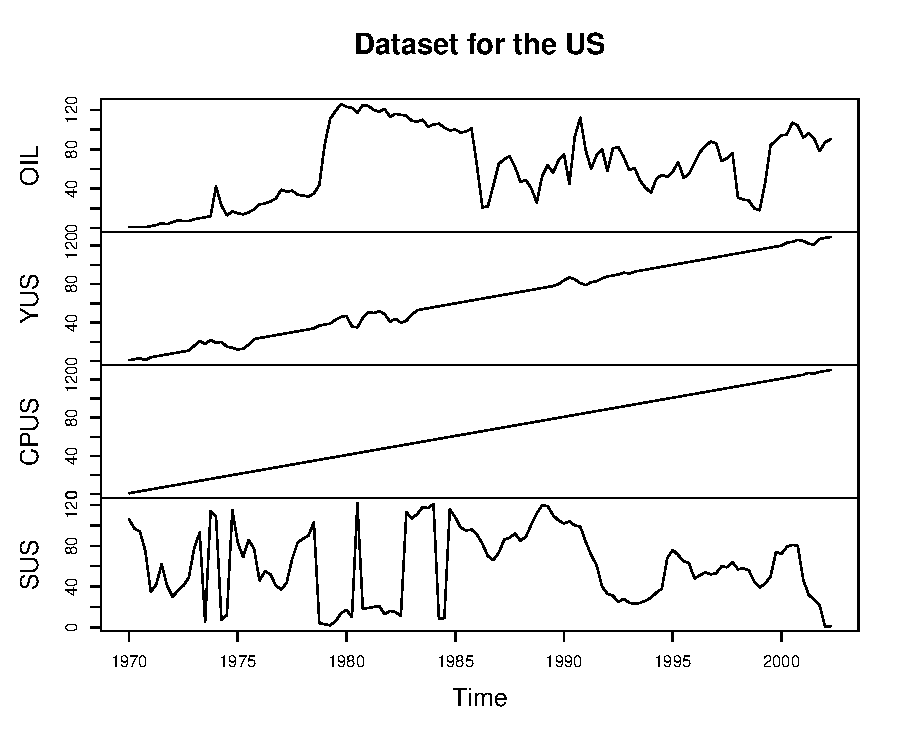
\includegraphics{replication_files/figure-latex/unnamed-chunk-5-1.pdf}

\begin{verbatim}
## NULL
\end{verbatim}

Now that I have a nice little graph, I can continue by creating my VAR.
WE first look at a simple four variable VAR. These variables are OIL,
CPUS, YUS and SUS. This VAR will then be used for my impulse response
functions.

\begin{verbatim}
## 
## VAR Estimation Results:
## ========================= 
## Endogenous variables: OIL, YUS, CPUS, SUS 
## Deterministic variables: const 
## Sample size: 129 
## Log Likelihood: -1390.997 
## Roots of the characteristic polynomial:
##     1 0.9102 0.6452 0.6452
## Call:
## VAR(y = ts_us, p = 1, type = "const")
## 
## 
## Estimation results for equation OIL: 
## ==================================== 
## OIL = OIL.l1 + YUS.l1 + CPUS.l1 + SUS.l1 + const 
## 
##         Estimate Std. Error t value Pr(>|t|)    
## OIL.l1   0.91555    0.03417  26.790   <2e-16 ***
## YUS.l1   0.54651    0.39879   1.370    0.173    
## CPUS.l1 -0.52412    0.39871  -1.315    0.191    
## SUS.l1  -0.03032    0.03407  -0.890    0.375    
## const    6.81916    3.50527   1.945    0.054 .  
## ---
## Signif. codes:  0 '***' 0.001 '**' 0.01 '*' 0.05 '.' 0.1 ' ' 1
## 
## 
## Residual standard error: 13.26 on 124 degrees of freedom
## Multiple R-Squared: 0.8771,  Adjusted R-squared: 0.8731 
## F-statistic: 221.2 on 4 and 124 DF,  p-value: < 2.2e-16 
## 
## 
## Estimation results for equation YUS: 
## ==================================== 
## YUS = OIL.l1 + YUS.l1 + CPUS.l1 + SUS.l1 + const 
## 
##          Estimate Std. Error t value Pr(>|t|)    
## OIL.l1  -0.002347   0.005720  -0.410    0.682    
## YUS.l1   0.682845   0.066743  10.231  < 2e-16 ***
## CPUS.l1  0.317619   0.066729   4.760  5.3e-06 ***
## SUS.l1   0.007525   0.005701   1.320    0.189    
## const    0.330629   0.586645   0.564    0.574    
## ---
## Signif. codes:  0 '***' 0.001 '**' 0.01 '*' 0.05 '.' 0.1 ' ' 1
## 
## 
## Residual standard error: 2.219 on 124 degrees of freedom
## Multiple R-Squared: 0.9966,  Adjusted R-squared: 0.9965 
## F-statistic:  9047 on 4 and 124 DF,  p-value: < 2.2e-16 
## 
## 
## Estimation results for equation CPUS: 
## ===================================== 
## CPUS = OIL.l1 + YUS.l1 + CPUS.l1 + SUS.l1 + const 
## 
##           Estimate Std. Error t value Pr(>|t|)    
## OIL.l1  -4.596e-05  5.657e-04  -0.081    0.935    
## YUS.l1   4.581e-03  6.601e-03   0.694    0.489    
## CPUS.l1  9.954e-01  6.600e-03 150.823   <2e-16 ***
## SUS.l1   9.405e-05  5.639e-04   0.167    0.868    
## const    1.000e+00  5.802e-02  17.238   <2e-16 ***
## ---
## Signif. codes:  0 '***' 0.001 '**' 0.01 '*' 0.05 '.' 0.1 ' ' 1
## 
## 
## Residual standard error: 0.2195 on 124 degrees of freedom
## Multiple R-Squared:     1,   Adjusted R-squared:     1 
## F-statistic: 9.279e+05 on 4 and 124 DF,  p-value: < 2.2e-16 
## 
## 
## Estimation results for equation SUS: 
## ==================================== 
## SUS = OIL.l1 + YUS.l1 + CPUS.l1 + SUS.l1 + const 
## 
##         Estimate Std. Error t value Pr(>|t|)    
## OIL.l1  -0.01602    0.07181  -0.223 0.823796    
## YUS.l1  -1.60957    0.83798  -1.921 0.057057 .  
## CPUS.l1  1.58774    0.83780   1.895 0.060404 .  
## SUS.l1   0.59208    0.07158   8.272 1.74e-13 ***
## const   24.97556    7.36556   3.391 0.000935 ***
## ---
## Signif. codes:  0 '***' 0.001 '**' 0.01 '*' 0.05 '.' 0.1 ' ' 1
## 
## 
## Residual standard error: 27.87 on 124 degrees of freedom
## Multiple R-Squared: 0.3841,  Adjusted R-squared: 0.3642 
## F-statistic: 19.33 on 4 and 124 DF,  p-value: 2.216e-12 
## 
## 
## 
## Covariance matrix of residuals:
##            OIL      YUS     CPUS       SUS
## OIL  175.87030  0.96627 -0.01711   4.93399
## YUS    0.96627  4.92607  0.05235  -2.04011
## CPUS  -0.01711  0.05235  0.04819   0.01546
## SUS    4.93399 -2.04011  0.01546 776.53784
## 
## Correlation matrix of residuals:
##            OIL      YUS      CPUS       SUS
## OIL   1.000000  0.03283 -0.005879  0.013351
## YUS   0.032829  1.00000  0.107433 -0.032985
## CPUS -0.005879  0.10743  1.000000  0.002528
## SUS   0.013351 -0.03299  0.002528  1.000000
\end{verbatim}

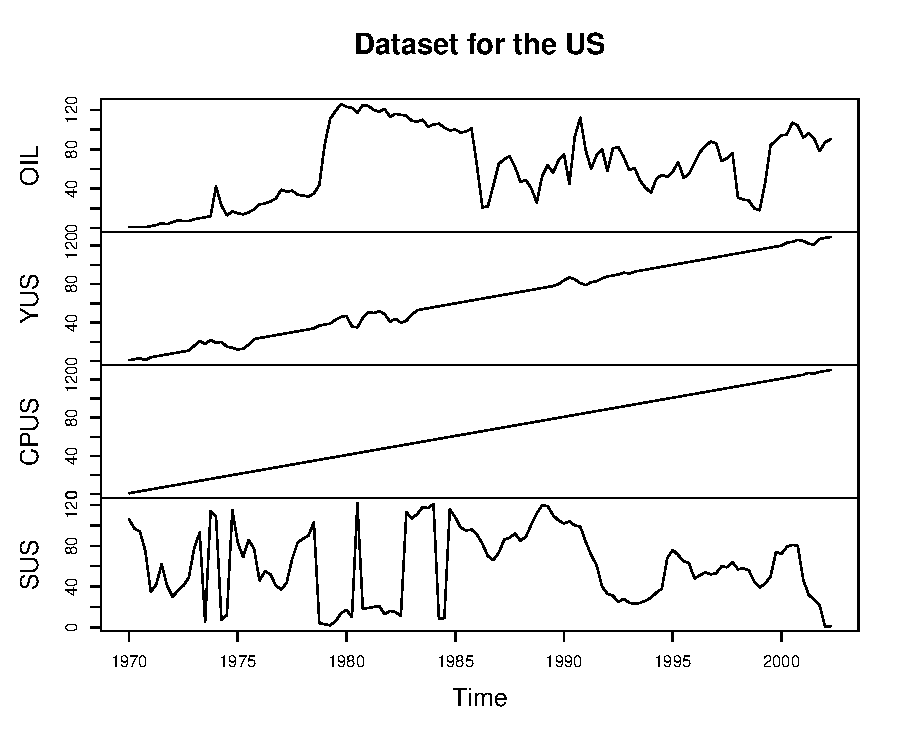
\includegraphics{replication_files/figure-latex/unnamed-chunk-6-1.pdf}
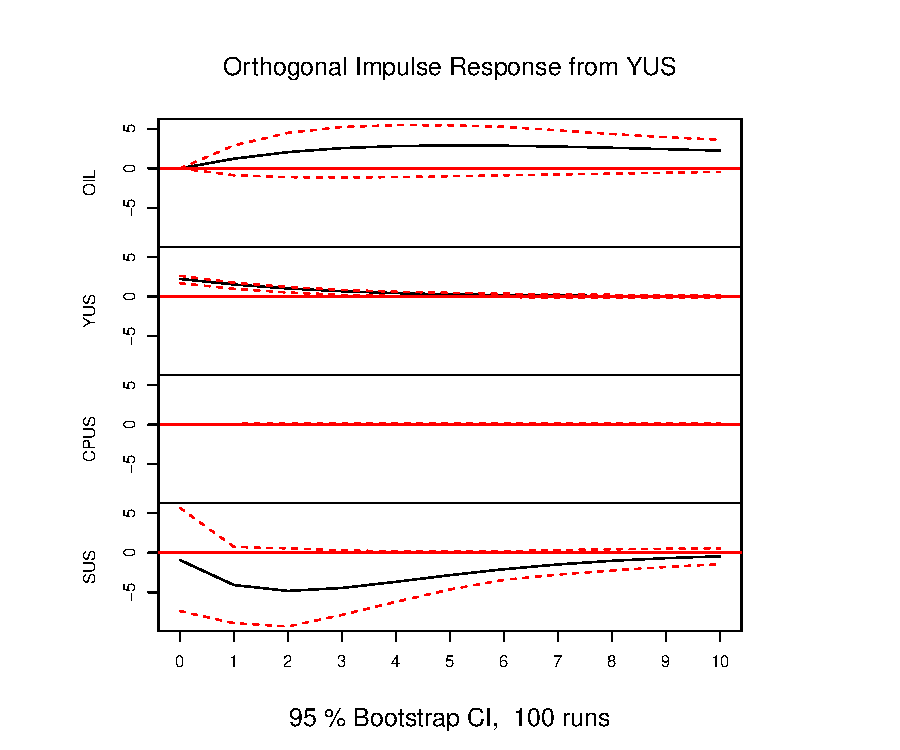
\includegraphics{replication_files/figure-latex/unnamed-chunk-6-2.pdf}
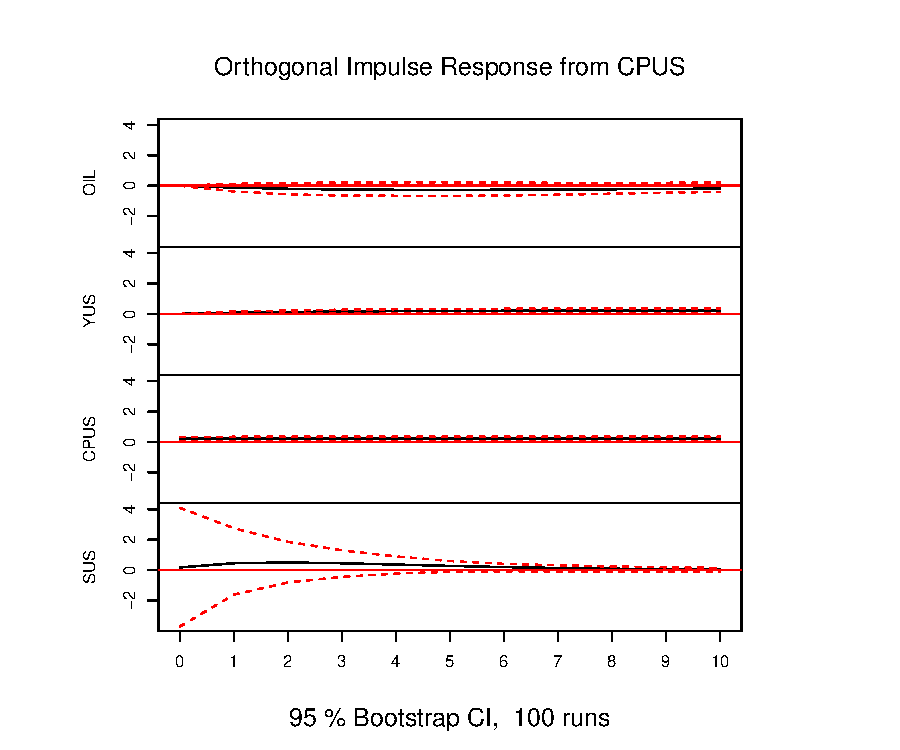
\includegraphics{replication_files/figure-latex/unnamed-chunk-6-3.pdf}
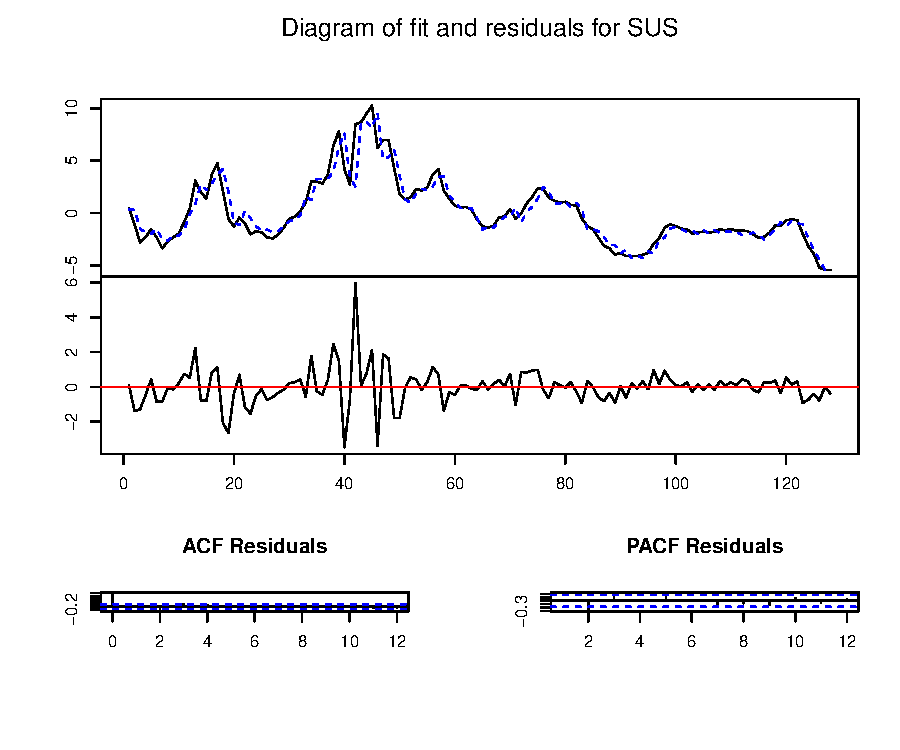
\includegraphics{replication_files/figure-latex/unnamed-chunk-6-4.pdf}

\hypertarget{conclusion}{%
\section{Conclusion}\label{conclusion}}

\newpage

\hypertarget{references}{%
\section*{References}\label{references}}
\addcontentsline{toc}{section}{References}

\hypertarget{refs}{}
\begin{CSLReferences}{0}{0}
\end{CSLReferences}

\hypertarget{appendix}{%
\section*{Appendix}\label{appendix}}
\addcontentsline{toc}{section}{Appendix}

\hypertarget{appendix-a}{%
\subsection*{Appendix A}\label{appendix-a}}
\addcontentsline{toc}{subsection}{Appendix A}

Some appendix information here

\hypertarget{appendix-b}{%
\subsection*{Appendix B}\label{appendix-b}}
\addcontentsline{toc}{subsection}{Appendix B}

\bibliography{Tex/ref}





\end{document}
